\documentclass[11pt,a4paper]{article}
\usepackage{iftex}
\ifXeTeX\usepackage{fontspec}\else\usepackage[T1]{fontenc}\usepackage[utf8]{inputenc}\fi
\usepackage[french]{babel}
\ifXeTeX\usepackage{microtype}\else\usepackage{lmodern,microtype}\fi
\usepackage[margin=2.3cm]{geometry}
\usepackage{amsmath,amssymb,amsthm}
\usepackage{graphicx,booktabs,float,caption,enumitem,xcolor}
\usepackage[hidelinks]{hyperref}
\usepackage{textcomp,newunicodechar}
\newunicodechar{→}{\ensuremath{\rightarrow}}
\newunicodechar{€}{\texteuro}
\newunicodechar{×}{\ensuremath{\times}}
\graphicspath{{../figures/}}
\setlist{itemsep=1pt,topsep=3pt}
\captionsetup{font=small,labelfont=bf}
\newtheorem*{prop}{Propriété}

\title{\textbf{Prévoir la baisse du Nikkei 225 : la régression logistique L2,}\\[2pt]
\large de la vraisemblance à la descente de gradient}
\author{Mathematics \& Statistics for Machine Learning (MSA-DATI07-04)\\ Albert School, MSc~1 --- Yann Linganzi, Arnault, Abhi, Fathi}
\date{Novembre 2026}

\begin{document}
\maketitle

\noindent\fbox{\parbox{\dimexpr\linewidth-2\fboxsep}{%
\textbf{Projet.} Chaque fin de mois, prédire la probabilité que le Nikkei 225 baisse le mois suivant, à partir de
variables de marché, de taux, de change et de news (février 2010 → septembre 2026). Ce rapport traite la partie
mathématique du modèle retenu ; la démarche complète d'apprentissage automatique (données, modèles, calibration, test,
explicabilité) est dans le rapport d'Applied ML.\\
\textbf{Dépôt Git :} \url{https://github.com/Thomaswayne2003/projetML}}}

\medskip


\noindent Le modèle du projet prédit, chaque fin de mois, la probabilité que le Nikkei 225 baisse le mois suivant. Ce
rapport dérive sa fonction de coût, son gradient et son prior de régularisation, puis analyse la sensibilité de son
optimisation. Le plan suit la recette de L1 : données, modèle, coût, optimiseur, évaluation. Les calculs sont dans
\texttt{notebooks/05\_annexe\_maths\_logistique.ipynb} et \texttt{src/logreg\_scratch.py}.

\section{Données et modèle}

On dispose de $m=143$ mois d'entraînement $(x^{(i)},y^{(i)})$, avec $x^{(i)}\in\mathbb R^{d}$, $d=12$ variables
standardisées (news, prix, taux, change, distances aux régimes k-means), et $y^{(i)}=1$ si le Nikkei baisse le mois
suivant. Le modèle est
\[
p^{(i)}=f_{w,b}\big(x^{(i)}\big)=\sigma\big(w^\top x^{(i)}+b\big),\qquad \sigma(u)=\frac{1}{1+e^{-u}} .
\]
En dérivant $\sigma(u)=(1+e^{-u})^{-1}$, on obtient
$\sigma'(u)=\dfrac{e^{-u}}{(1+e^{-u})^2}=\sigma(u)\big(1-\sigma(u)\big)$, propriété qui rendra le gradient très simple.

\section{Le coût, par maximum de vraisemblance}

Chaque mois est un tirage de Bernoulli de paramètre $p^{(i)}$ : $P(y^{(i)}\mid x^{(i)})=(p^{(i)})^{y^{(i)}}(1-p^{(i)})^{1-y^{(i)}}$.
En supposant les mois indépendants, la vraisemblance est un produit ; on maximise son logarithme, ce qui revient à
minimiser la log-loss :
\[
J(w,b)=-\frac1m\log\prod_{i=1}^{m}P\big(y^{(i)}\mid x^{(i)}\big)
=-\frac1m\sum_{i=1}^{m}\Big[y^{(i)}\log p^{(i)}+\big(1-y^{(i)}\big)\log\big(1-p^{(i)}\big)\Big].
\]
\emph{Hypothèse à discuter.} Les rendements mensuels successifs sont peu corrélés mais pas exactement indépendants :
la vraisemblance est une approximation.

\section{Le gradient}

Pour un mois, avec $u=w^\top x+b$ et $J_i$ le terme de la somme, la règle de la chaîne donne
\[
\frac{\partial J_i}{\partial w_j}
=\underbrace{\Big(-\frac{y}{p}+\frac{1-y}{1-p}\Big)}_{\partial J_i/\partial p}
\cdot\underbrace{p(1-p)}_{\partial p/\partial u}\cdot\underbrace{x_j}_{\partial u/\partial w_j}
=\big(-y(1-p)+(1-y)p\big)x_j=(p-y)\,x_j .
\]
D'où, sous forme matricielle ($X\in\mathbb R^{m\times d}$, $p,y\in\mathbb R^m$) :
\[
\nabla_w J=\frac1m X^\top(p-y),\qquad \frac{\partial J}{\partial b}=\frac1m\sum_{i=1}^m\big(p^{(i)}-y^{(i)}\big).
\]
C'est la forme de la régression linéaire de L1 : l'erreur de prédiction fois l'entrée. \textbf{Vérification
numérique} : en un point tiré au hasard, le gradient analytique et les différences finies centrées
$\big(J(w+\varepsilon e_j)-J(w-\varepsilon e_j)\big)/2\varepsilon$ s'accordent à $1{,}3\times10^{-9}$ près (écart relatif).

\section{La régularisation L2 comme prior gaussien}

On suppose a priori $w\sim\mathcal N(0,\tau^2 I)$. Maximiser la probabilité a posteriori (MAP) revient à ajouter
$-\frac1m\log p(w)$ au coût :
\begin{gather*}
-\frac1m\log p(w)=\frac{\lVert w\rVert_2^2}{2m\tau^2}+\text{cste}
\quad\Longrightarrow\quad
J_\lambda(w,b)=J(w,b)+\lambda\lVert w\rVert_2^2,\qquad \lambda=\frac{1}{2m\tau^2},\\
\nabla_wJ_\lambda=\frac1mX^\top(p-y)+2\lambda w .
\end{gather*}
\begin{itemize}
\item L'intercept $b$ n'a pas de prior : il n'est pas pénalisé. Le solveur \texttt{liblinear} le pénalise et tirait les
probabilités vers 50~\% ; le projet utilise donc \texttt{saga}.
\item scikit-learn minimise $\tfrac12\lVert w\rVert^2+C\sum_i\ell_i$ ; en divisant par $Cm$, on retrouve $J_\lambda$ avec
$\lambda=1/(2mC)$. Le $C=0{,}0299$ choisi par Optuna donne $\lambda=0{,}117$, soit un écart-type a priori
$\tau=0{,}17$ par poids standardisé : avant de voir les données, on juge qu'un écart-type de plus sur une variable change
le log-odds de la baisse de moins de $0{,}35$ environ, dans 95~\% des cas.
\end{itemize}

\begin{prop}[convexité stricte]
La hessienne de $J_\lambda$ par rapport à $(w,b)$ vaut
$H=\frac1m\tilde X^\top S\tilde X+2\lambda\,\mathrm{diag}(1,\dots,1,0)$, avec $\tilde X=[X,\mathbf 1]$ et
$S=\mathrm{diag}\big(p^{(i)}(1-p^{(i)})\big)$. Pour $(v,c)\neq0$,
$(v,c)^\top H(v,c)=\frac1m(Xv+c\mathbf 1)^\top S(Xv+c\mathbf 1)+2\lambda\lVert v\rVert^2>0$ : si $v\neq0$ le second terme
est strictement positif, et si $v=0$ le premier vaut $\frac{c^2}m\sum_i p^{(i)}(1-p^{(i)})>0$. $J_\lambda$ est donc
strictement convexe et admet un minimum unique.
\end{prop}

\section{L'optimiseur : la descente de gradient}

\[
w\leftarrow w-\alpha\,\nabla_wJ_\lambda(w,b),\qquad b\leftarrow b-\alpha\,\frac{\partial J_\lambda}{\partial b},\qquad\text{départ } (w,b)=(0,0).
\]
\textbf{Choix du pas.} Comme $p(1-p)\le\frac14$, le gradient de $J_\lambda$ est $L$-lipschitzien avec
$L\le\frac14\lambda_{\max}\big(\tilde X^\top\tilde X/m\big)+2\lambda=0{,}962$ sur nos données. Le pas classique est
$\alpha=1/L=1{,}04$, et la descente converge pour tout $\alpha<2/L=2{,}08$.

\begin{table}[H]\centering\small
\begin{tabular}{lccc}\toprule
Paramètre & Descente à la main & scikit-learn \texttt{lbfgs} & Modèle final (\texttt{saga}) \\\midrule
$w_1$ (volume anormal d'articles) & 0,20033 & 0,20033 & 0,20033 \\
$w_4$ (momentum 12 mois) & 0,20212 & 0,20212 & 0,20212 \\
$w_7$ (variation du JGB 10 ans) & 0,10566 & 0,10566 & 0,10567 \\
$b$ & $-0{,}45359$ & $-0{,}45359$ & $-0{,}45352$ \\\midrule
Écart maximal sur les 13 paramètres & --- & $4{,}6\times10^{-6}$ & $7{,}3\times10^{-5}$ \\\bottomrule
\end{tabular}
\caption{La descente codée à la main ($\alpha=1/L$, 20\,000 itérations) retrouve scikit-learn. Au point trouvé, $\lVert\nabla J_\lambda\rVert=1{,}5\times10^{-17}$ :
la condition d'optimalité est vérifiée.}
\end{table}

\section{Analyse de sensibilité de l'optimisation}

\paragraph{Le pas $\alpha$.} La borne $2/L=2{,}08$ est prudente : la limite locale, calculée avec la hessienne au
minimum, vaut $2/\lambda_{\max}(H^\ast)=2{,}23$, parce que $p(1-p)$ reste nettement sous $\frac14$. La descente est
lente pour $\alpha=0{,}01$ (encore $2\times10^{-8}$ d'écart à $J^\ast$ après 3\,000 itérations), converge de
$\alpha=0{,}1$ à $0{,}95\times2{,}23$, d'autant plus vite que $\alpha$ est grand, et ne converge plus à
$1{,}2\times2{,}23$ (écart bloqué à 0,22).

\begin{figure}[H]\centering
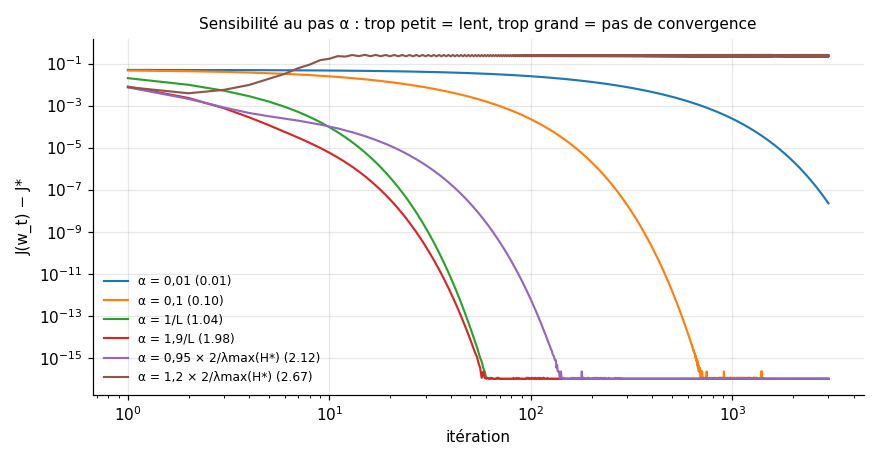
\includegraphics[width=.49\linewidth]{05_sensibilite_pas.png}\hfill
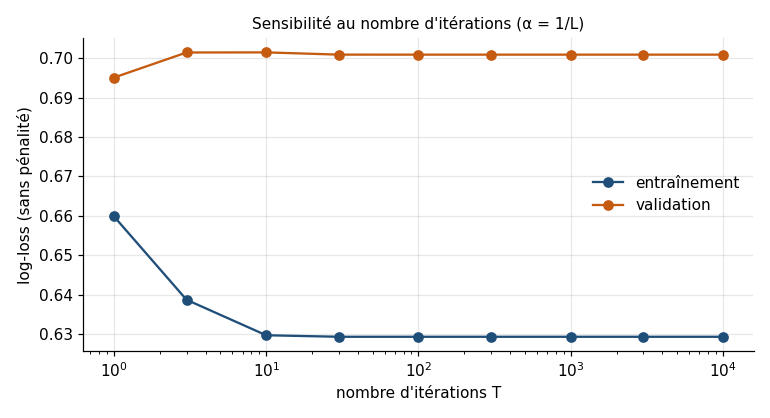
\includegraphics[width=.49\linewidth]{05_sensibilite_iterations.png}
\caption{À gauche, $J(w_t)-J^\ast$ selon le pas : trop petit = lent, trop grand = pas de convergence. À droite,
log-loss d'entraînement et de validation selon le nombre d'itérations ($\alpha=1/L$).}
\end{figure}

\paragraph{Le nombre d'itérations.} Avec $\alpha=1/L$, la descente converge en une trentaine d'itérations. La
log-loss de validation est la plus basse dès la première itération (0,695 contre 0,701 à convergence) : arrêter tôt
garde les poids près de 0, donc régularise. C'est cohérent avec le peu de signal stable du problème.

\paragraph{La force $\lambda$ (compromis biais-variance, S3).} Sans pénalité, la log-loss d'entraînement est la plus
basse (0,606) mais celle de validation croisée temporelle monte à 0,766 et celle de validation à 0,882 :
sur-apprentissage. La validation croisée est minimale au $\lambda$ choisi par Optuna (0,650 ; l'écart avec le 0,647
d'Optuna vient de $\lambda=1/(2mC)$, calculé avec $m=143$ alors que les folds comptent 95 à 131 mois). Sur la validation
2022-2023, c'est le plus grand $\lambda$ testé qui gagne (0,680), presque le modèle constant.

\paragraph{Le point de départ.} Trois départs très différents ($J$ initial entre 0,69 et 12,4) mènent au même minimum
à $10^{-17}$ près : c'est la convexité stricte, observée en pratique.

\begin{figure}[H]\centering
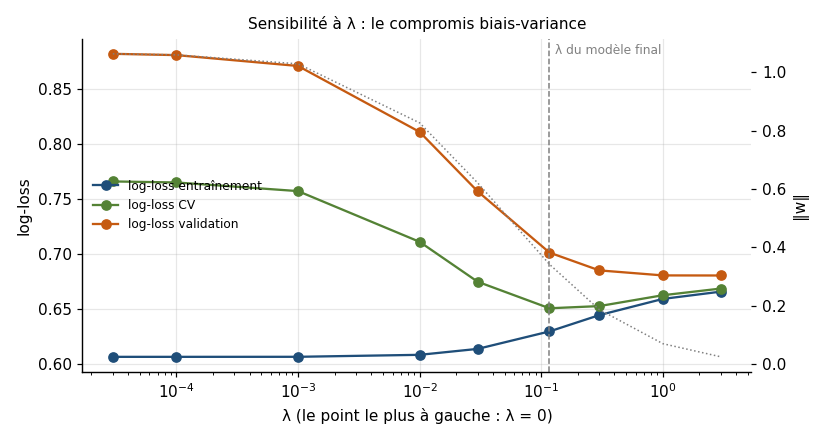
\includegraphics[width=.49\linewidth]{05_sensibilite_lambda.png}\hfill
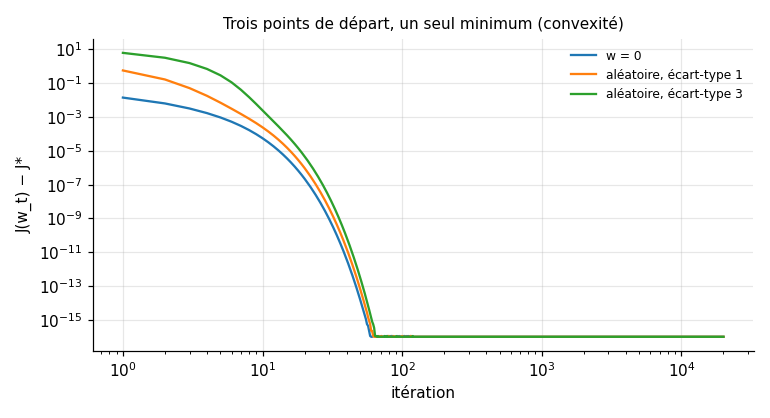
\includegraphics[width=.49\linewidth]{05_sensibilite_depart.png}
\caption{À gauche, log-loss d'entraînement, de validation croisée et de validation, et $\lVert w\rVert$, selon
$\lambda$. À droite, trois points de départ, un seul minimum.}
\end{figure}

\section{Et une régression sur le rendement ? (L2)}

Avec les mêmes 12 variables, les équations normales $\tilde X^\top\tilde X\beta=\tilde X^\top r$, résolues à la main,
retrouvent scikit-learn à $10^{-16}$ près. Le $R^2$ vaut 0,12 sur l'entraînement mais $-1{,}77$ sur la validation :
prédire le montant du rendement est hors de portée, ce qui justifie le passage à la classification.

\section*{Ce qu'il faut retenir}

La log-loss est l'opposé de la log-vraisemblance de Bernoulli ; son gradient est $\frac1mX^\top(p-y)$ ; la pénalité
L2 est un prior gaussien de variance $\tau^2=1/(2m\lambda)$ qui rend le problème strictement convexe ; la descente de
gradient converge pour $\alpha<2/L$ et retrouve scikit-learn. Sur ce problème, toutes les sensibilités pointent dans le
même sens : plus de régularisation, ou un arrêt plus précoce, rapproche le modèle de la constante, signe d'un signal
faible et instable dans le temps.

% Rôles des membres et usage de l'IA : partie commune aux deux rapports (% Rôles des membres et usage de l'IA : partie commune aux deux rapports (% Rôles des membres et usage de l'IA : partie commune aux deux rapports (\input{roles_et_ia}).

\section*{Contributions des membres}

\begin{table}[H]\centering\small
\begin{tabular}{p{3.2cm}p{12cm}}\toprule
Membre & Ce qu'il a fait \\\midrule
\textbf{Yann Linganzi} &
\textbf{Conception et conduite du projet.} Choix de la question (acheter, rester neutre ou vendre le Nikkei, couvert
ou non contre le yen) et de sa traduction en deux classifications ; collecte des données (versions 1 et 2), choix des
sources et des décalages de publication ; audit des fuites ; exploration et construction des variables ; découpage
chronologique ; pipeline, trois modèles et réglage Optuna ; choix de la log-loss comme critère ; calibration de Platt
et règle de décision par espérance de gain, figées avant le test ; évaluation unique du test ; explicabilité
(tranches, permutation, SHAP, dépendances partielles) ; annexe mathématique (logistique codée à la main, sensibilité,
moindres carrés) ; seconde version 1999-2026 avec le contrôle des séries Bloomberg ; explorations après coup et
protocole figé de la troisième version ; API, tableau de bord et site ; rédaction des rapports. \\[3pt]
\textbf{arnshl} &
Captures du terminal Bloomberg (huit écrans : inflation japonaise, fondamentaux et décomposition du rendement du
Nikkei, révisions des bénéfices, rendement des bénéfices contre le taux américain à 10 ans, trajectoires du bénéfice
par action), avec les vérifications visuelles et les pistes de variables qu'elles suggèrent ; chiffres qui justifient
les conclusions des salles III et VII du site ; relecture et fusion des contributions sur GitHub. \\[3pt]
\textbf{jovi-mce} &
Version anglaise du site (\texttt{site/en/}) et sa mise en ligne. \\\bottomrule
\end{tabular}\end{table}

\section*{Usage de l'IA}

La réflexion et la méthode sont les nôtres. Yann Linganzi a posé le problème et décidé de chaque choix de méthode :
les variables et leurs dates de publication, le découpage dans le temps, les modèles comparés, le critère, la
calibration, la règle de décision et l'engagement pris avant d'ouvrir le test, puis, après coup, les vérifications à
mener et le protocole de la troisième version. Il a testé chacun de ces choix et validé chaque résultat : audit des
fuites, vérifications qui retrouvent à l'identique la décision et l'évaluation figées, tests automatiques, lecture et
interprétation des chiffres.

Un assistant IA (Claude, d'Anthropic) a servi d'aide à la programmation : écriture du code Python des modules et des
notebooks à partir de ces choix, mise en forme du site et des figures, et aide à la relecture et à la mise en forme de
la rédaction. Tout ce qu'il a produit a été relu, exécuté et vérifié avant d'être gardé ; quand un résultat ne
tenait pas, c'est la méthode qui a été corrigée, pas le chiffre. La soutenance est assurée par le groupe.
).

\section*{Contributions des membres}

\begin{table}[H]\centering\small
\begin{tabular}{p{3.2cm}p{12cm}}\toprule
Membre & Ce qu'il a fait \\\midrule
\textbf{Yann Linganzi} &
\textbf{Conception et conduite du projet.} Choix de la question (acheter, rester neutre ou vendre le Nikkei, couvert
ou non contre le yen) et de sa traduction en deux classifications ; collecte des données (versions 1 et 2), choix des
sources et des décalages de publication ; audit des fuites ; exploration et construction des variables ; découpage
chronologique ; pipeline, trois modèles et réglage Optuna ; choix de la log-loss comme critère ; calibration de Platt
et règle de décision par espérance de gain, figées avant le test ; évaluation unique du test ; explicabilité
(tranches, permutation, SHAP, dépendances partielles) ; annexe mathématique (logistique codée à la main, sensibilité,
moindres carrés) ; seconde version 1999-2026 avec le contrôle des séries Bloomberg ; explorations après coup et
protocole figé de la troisième version ; API, tableau de bord et site ; rédaction des rapports. \\[3pt]
\textbf{arnshl} &
Captures du terminal Bloomberg (huit écrans : inflation japonaise, fondamentaux et décomposition du rendement du
Nikkei, révisions des bénéfices, rendement des bénéfices contre le taux américain à 10 ans, trajectoires du bénéfice
par action), avec les vérifications visuelles et les pistes de variables qu'elles suggèrent ; chiffres qui justifient
les conclusions des salles III et VII du site ; relecture et fusion des contributions sur GitHub. \\[3pt]
\textbf{jovi-mce} &
Version anglaise du site (\texttt{site/en/}) et sa mise en ligne. \\\bottomrule
\end{tabular}\end{table}

\section*{Usage de l'IA}

La réflexion et la méthode sont les nôtres. Yann Linganzi a posé le problème et décidé de chaque choix de méthode :
les variables et leurs dates de publication, le découpage dans le temps, les modèles comparés, le critère, la
calibration, la règle de décision et l'engagement pris avant d'ouvrir le test, puis, après coup, les vérifications à
mener et le protocole de la troisième version. Il a testé chacun de ces choix et validé chaque résultat : audit des
fuites, vérifications qui retrouvent à l'identique la décision et l'évaluation figées, tests automatiques, lecture et
interprétation des chiffres.

Un assistant IA (Claude, d'Anthropic) a servi d'aide à la programmation : écriture du code Python des modules et des
notebooks à partir de ces choix, mise en forme du site et des figures, et aide à la relecture et à la mise en forme de
la rédaction. Tout ce qu'il a produit a été relu, exécuté et vérifié avant d'être gardé ; quand un résultat ne
tenait pas, c'est la méthode qui a été corrigée, pas le chiffre. La soutenance est assurée par le groupe.
).

\section*{Contributions des membres}

\begin{table}[H]\centering\small
\begin{tabular}{p{3.2cm}p{12cm}}\toprule
Membre & Ce qu'il a fait \\\midrule
\textbf{Yann Linganzi} &
\textbf{Conception et conduite du projet.} Choix de la question (acheter, rester neutre ou vendre le Nikkei, couvert
ou non contre le yen) et de sa traduction en deux classifications ; collecte des données (versions 1 et 2), choix des
sources et des décalages de publication ; audit des fuites ; exploration et construction des variables ; découpage
chronologique ; pipeline, trois modèles et réglage Optuna ; choix de la log-loss comme critère ; calibration de Platt
et règle de décision par espérance de gain, figées avant le test ; évaluation unique du test ; explicabilité
(tranches, permutation, SHAP, dépendances partielles) ; annexe mathématique (logistique codée à la main, sensibilité,
moindres carrés) ; seconde version 1999-2026 avec le contrôle des séries Bloomberg ; explorations après coup et
protocole figé de la troisième version ; API, tableau de bord et site ; rédaction des rapports. \\[3pt]
\textbf{arnshl} &
Captures du terminal Bloomberg (huit écrans : inflation japonaise, fondamentaux et décomposition du rendement du
Nikkei, révisions des bénéfices, rendement des bénéfices contre le taux américain à 10 ans, trajectoires du bénéfice
par action), avec les vérifications visuelles et les pistes de variables qu'elles suggèrent ; chiffres qui justifient
les conclusions des salles III et VII du site ; relecture et fusion des contributions sur GitHub. \\[3pt]
\textbf{jovi-mce} &
Version anglaise du site (\texttt{site/en/}) et sa mise en ligne. \\\bottomrule
\end{tabular}\end{table}

\section*{Usage de l'IA}

La réflexion et la méthode sont les nôtres. Yann Linganzi a posé le problème et décidé de chaque choix de méthode :
les variables et leurs dates de publication, le découpage dans le temps, les modèles comparés, le critère, la
calibration, la règle de décision et l'engagement pris avant d'ouvrir le test, puis, après coup, les vérifications à
mener et le protocole de la troisième version. Il a testé chacun de ces choix et validé chaque résultat : audit des
fuites, vérifications qui retrouvent à l'identique la décision et l'évaluation figées, tests automatiques, lecture et
interprétation des chiffres.

Un assistant IA (Claude, d'Anthropic) a servi d'aide à la programmation : écriture du code Python des modules et des
notebooks à partir de ces choix, mise en forme du site et des figures, et aide à la relecture et à la mise en forme de
la rédaction. Tout ce qu'il a produit a été relu, exécuté et vérifié avant d'être gardé ; quand un résultat ne
tenait pas, c'est la méthode qui a été corrigée, pas le chiffre. La soutenance est assurée par le groupe.


\end{document}
